\section{Modular vs End-to-End Approaches}

When developing systems for autonomous driving, we generally differ between two main approaches: modular and end-to-end \cite{multimodal-e2e-ad}. The former divides the autonomous system into modules with different areas of responsibility. There can for example be different modules responsible for perception, prediction, route planning or vehicle control. These modules vary in complexity. The end-to-end approach on the other hand looks at the autonomous system as one complete unit. This approach maps raw sensor data (RGB camera, LIDAR, GPS, etc.) directly into actions (acceleration, steering, braking, etc.). A visual comparision of the two approacches can be seen in \cref{fig:modular-vs-end-to-end}.

\begin{figure}[htbp]
    \centering
    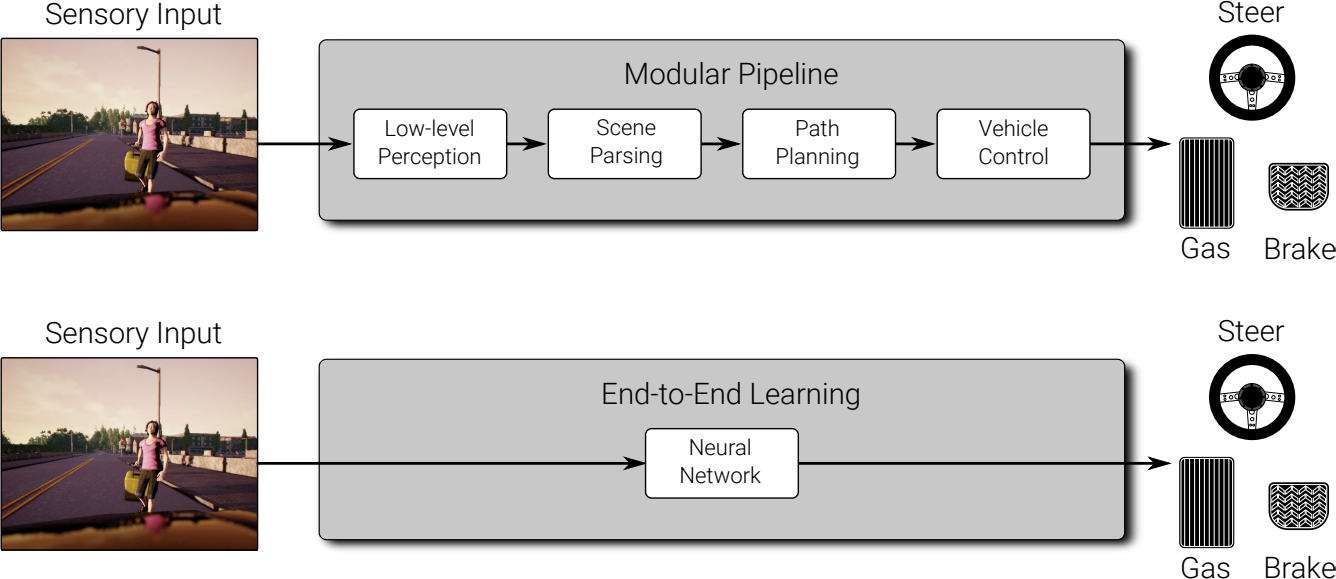
\includegraphics[width=\textwidth]{figures/2/modular-end-to-end.png}
    \caption{Figure showing the difference between modular (top) and end-to-end (bottom) approaches to autonomous vehicles. Source: \cite{computer-vision-for-autonomous-vehicles}.}
    \label{fig:modular-vs-end-to-end}
\end{figure}

As discussed in a recent paper comparing end-to-end techniques, there is an ongoing shift towards the latter approach \cite{survey-on-end-to-end-techniques}. Even though the modular approach offers an explainable and verifiable system where each module can individually be evaluated, it lacks efficient use of computer resources and awareness of the high-level task that is autonomous driving. In addition, the modular approach requires huge amount of annotated data for each module. This is in contrast to the end-to-end approach where the annotations lives in the state of the car (steering commands, GPS location, etc.) at a given moment. This approach does however require the sensors to be synchronized. 
